%Kapitel der Umsetzung

\chapter{OSINT einer ausgewählten Person}  %Name des Kapitels
\label{cha:Informationsbeschaffung einer ausgewählten Person} %Label des Kapitels

\section{Auswahl der Programmiersprache}
Damit das Programm anhand den Lösungsideen umgesetzt werden kann, ist der erste Schritt die Auswahl der Programmiersprache.\\
Hierbei wird keine Anforderung an die Geschwindigkeit der Sprache gestellt, da beim web scraping das Internet den zeitlichen Engpass darstellt. Allerdings wäre es von Vorteil wenn bereits entwickelte Bibliotheken für das web scraping vorhanden sind. Die Eingabe der Information für die Suche kann über eine Konsole oder über eine graphische Benutzeroberfläche möglich sein.\\
Als mögliche Programmiersprachen zählen Python, Ruby, C++.\\
Für web-basierende Anwendung eignet sich eine dynamische Programmsprache.
Im Gegensatz zu Python und Ruby zählt C++ nicht zur Familie der dynamischen Programmiersprachen und fällt aus diesem Grund als mögliche Lösung heraus. \\
Python und Ruby können beide Webseiten, die JavaScript zum rendern benötigen, laden. Dies ist mit Hilfe eines automatisierten Webbrowsers möglich. Des Weiteren lässt sich die Anwendung durch beide Sprachen, entsprechend den Anforderungen entwickeln. Es kann sowohl eine Oberflächenanwendung als auch eine Konsolenanwendung programmiert werden. Zusätzlich bringen beide Sprachen Module mit sich, um das Pojekt mit den vorgegebenen Zielen umzusetzen. Somit haben beide Programmiersprachen die Voraussetzungen für die Entwicklung der Anwendung. Allerdings bietet Python in diesem Bereich eine große Community und eignet sich sehr gut für die Bearbeitung von linguistischen Daten. \cite{bird2009natural}
Aus diesen Gründen wird die zu erstellende Anwendung mit der Programmiersprache Python entwickelt.


%TODO Scrapy Beautiful Soup
	
\section{Methoden zur Suche nach einer Person im Internet}
\label{sec:Suche nach Information}
Für die Suche einer Person im Internet, wird abhängig von den eingegebenen Daten, des Programm-Anwenders, die Art der Suche angepasst. Das heißt, dass die eingegebenen Daten vor der Suche analysiert werden und dementsprechend die Suche danach angepasst wird. \\
Die Art der Personensuche lässt sich in zwei mögliche Methoden gliedern.

	\subsection{Personensuche mit Hilfe einer Suchmaschine}
	\label{subsubsec:PersonensucheMitHilfevonSuchmaschine}
	Hier wird mit Hilfe einer Suchmaschine nach Informationen gesucht. Mögliche Suchmaschinen sind die von Google und Bing. Allerdings muss nicht für jede Suche eine Suchmaschine verwendet werden. Die nachfolgenden Fälle sollen diesen Ansatz verdeutlichen.
	
	Im Fall, dass der Vorname, Nachname und Wohnort der gesuchten Person eingegeben wird, kann mit Hilfe der festgelegten Suchmaschine nach Information gesucht werden. Die von den Suchmaschinen vorgeschlagenen Seiten werden anschließend analysiert, ausgelesen und gespeichert. Dadurch können weitere Informationen gewonnen werden. Falls Benutzernamen von anderen Webseiten wie Instagram, Facebook oder ähnliches vorgeschlagen werden, kann somit die Suche mit diesen Daten speziell auf den entsprechenden Seiten erweitert werden.
	
	Ein weiterer Fall beschreibt das Szenario, wenn ein Benutzername der gesuchten Person in das Programm eingegeben wird. Hierbei handelt es sich um einen Benutzernamen von Social-Media-Webseiten wie Facebook, Instagram, LinkedIn, et cetera. \\
	Zuallererst, wird hier nach Einträgen auf der entsprechende Webseite zu dem angegebenen Benutzername durchsucht. Dadurch können zusätzliche Daten herausgefunden werden, die bei der weiteren Suche von Vorteil sind.\\
	Sobald die Webseite mit Hilfe des Nutzernamens durchsucht und ausgewertet wurde, kann die Suche mit einer Suchmaschine erweitert werden.
	
	\subsection{Personensuche auf festgelegten Webseiten}
	\label{subsubsec:PersonensucheohneSuchmaschine}
	Unabhängig von den eingegebenen Daten, wird eine festgesetzte Anzahl von Webseiten durchsucht. Als potentielle Kandidaten-Webseiten eigenen sich die Social-Media-Seiten wie Facebook, Instagram, Twitter, LinkedIn, et cetera. Diese Art der Personensuche arbeitet allerdings ohne die Verwendung einer Suchmaschine.
	
\section{Bewertung: Art der Personensuche}
Um möglichst viele Informationen über eine Person im Internet zu finden, bietet die Personensuche mit der Verwendung einer Suchmaschine die beste Lösung. Es wird anstatt ausschließlich festgelegten Seiten das ganze Internet durchsucht. Dadurch können wesentlich mehr individuelle Einträge gefunden werden. Des Weiteren wird keine Logik zur Suche nach Einträgen im Internet benötigt, da lediglich den vorgeschlagenen Suchergebnissen gefolgt werden kann.\\
Allerdings muss beachtet werden, dass Benutzer bei verschiedensten Social-Media-Seiten auswählen können, ob das Benutzerprofil von einer Suchmaschine gefunden werden kann oder nicht. Aus diesem Grund, werden bei dieser Suche die Ergebnisse kontrolliert ob sich die geforderten Seiten darin befinden. Wenn das nicht der Fall ist, wird separat auf den festgelegten Seiten nach Information gesucht. Bekannte Webseiten die diese Einstellungsmöglichkeiten unterstützen XING und LinkedIn.\\
	\subsection{Auswahl der Suchmaschine}
	%TODO Google oder Bing?!
	Laut Expertenaussage sucht Bing tiefgreifender nach Information auf Social Media Seiten wie Facebook, Twitter und LinkedIn. Allerdings finden nur 3,5\% aller Suchanfragen in Deutschland über Bing statt. Im Gegensatz dazu hat Google einen Marktanteil von 91,2\% in Deutschland. Diese Zahlen sprechen eindeutig für Google. Durch die höhere Anzahl von Suchanfragen, können mehr Daten erfasst und die Ergebnislisten besser gerankt werden. Dies hat zu Folge, dass Bing bei einer konkreten Suche schlechter abschneidet. \cite{Suchmaschinen}
	Grundsätzlich stellt die Verwendung von zwei Suchmaschinen die beste Lösung dar, da die Wahrscheinlichkeit für einen Suchtreffer erhöht wird. Dennoch wird in dieser Arbeit ausschließlich die Suchmaschine von Google verwendet, da sie gegenüber dem Konkurrenten keine Nachteile hat. Selbst die detailliertere Suche auf Sozialen Netzwerken, bringt bei der hier verwendeten Personensuche keinen großen Vorteil für Bing. Das heißt, durch die Analyse der Suchergebnisse, wird erkannt ob sich die bekannten Social Media Webseiten darunter befinden. Falls diese es nicht tun, wird die Suche auf den entsprechenden Sozialen Netzwerken erweitert.
	 	
\section{Umsetzung: Personensuche mit Hilfe der Google-Suchmaschine im Internet}
Für die Personensuche im Internet wird die Google-Suchmaschine verwendet. Gesucht wird nach den eingegebenen Daten, welche über die Konsole eingelesen werden.

	\subsection{Eingabe der bekannten Daten}
	Es besteht die Möglichkeit den \textbf{Vorname, Nachname, Wohnort, Arbeitgeber, Instagram Benutzername, Facebook Benutzername, Twitter Benutzername}, und das genaue beziehungsweise geschätzte \textbf{Geburtsjahr} der gesuchten Person über eine Konsole einzugeben. Falls der genaue Jahrgang der Zielperson nicht bekannt ist, kann ein geschätztes Geburtsjahr eingetragen werden. Dies kann später bei der Identifizierung der gesuchten Person hilfreich sein.\\
	Zu Beginn werden alle Personen-Variablen mit einem leeren String initialisiert. Das bedeutet, alle Variablen, zu denen keine Information eingegeben wurde, enthalten einen leeren String.
	
		\subsubsection{Verarbeitung der Daten}
		Zu Beginn der Anwendung werden Abfragen gemacht, um zu erkennen in welchen Variablen sich Information befindet. Dabei kann gleichzeitig die Eingabe des Wohnortes mit der entsprechenden Wortsammlung verglichen werden. Falls sich der Wohnort nicht in der Datenbank befindet, kann er nachträglich ergänzt werden. Dies könnte bei der Informationserkennung von Vorteil sein.\\
		Daraufhin werden mit diesen Eingaben Kombinationen für die Suche und die URL-Generierung erstellt. Mögliche Such-Kombinationen für erfolgreiche Ergebnisse sind:
		
		\textit{Vorname, Nachname, Wohnort;}\\
		\textit{Vorname, Nachname, Geburtsjahr;}\\
		\textit{Vorname, Nachname, Institution;}\\
		\textit{Vorname, Nachname, Wohnort, Geburtsjahr;}\\
		\textit{Vorname, Nachname, Wohnort, Institution;}\\
		\textit{Benutzername einer Social-Media-Seite;}
		
		
		Die Kombination aus vielen oder allen Daten ist ebenfalls eine mögliche Option, allerdings wird dadurch oft kein Ergebnis gefunden, da nicht zur jeder Information ein Eintrag im Internet besteht.\\
		Sobald die Kombinationen aus den Daten bekannt sind, werden die Such-URLs für die Google-Suchmaschine generiert.
		\subsection{Erstellen der Such-URLs}	
			\subsubsection{Aufbau eines URLs}
			\label{subsec:AufbauURL}
			Ein Uniform Resource Locator, kurz URL, lokalisiert eine Ressource, indem eine abstrakte Identifikation der Lokalisierung verwendet wird. Dabei wird ein URL grundsätzlich im folgenden Format angegeben.\cite{RFC1738}
			
			$<scheme>:<scheme-specific-part>$ \cite{RFC1738}
			
			Das Schema gleicht hierbei meist dem verwendeten Protokoll wie HTTP oder FTP. Der Doppelpunkt stellt die Trennung zum Schema-spezifischen Teil dar. Ein Beispiel für ein HTTP-URL-Aufbau ist im Folgenden definiert.\cite{RFC1738}
			
			$http://<host>:<port>/<path>?<searchpart>$\cite{RFC1738}
			
			Hier wird das Protokoll HTTP als Schema verwendet, wobei sich der Aufbau bei der Verwendung des HTTPS-Protokolls kaum unterscheidet. Lediglich das Schema und der Port verändert sich.\\
			Für den <host> kann der FQDN oder die IP-Adresse des Hostrechners eingetragen werden. Wenn der Port nicht angegeben wird, ist der Standardport voreingestellt. Bei HTTP wäre dies Port 80 und bei HTTPS Port 443. Der <path> stellt ein HTTP-Selektor dar und ist mit einem Fragezeichen von der Suchzeichenkette getrennt.\cite{RFC1738}\\ %TODO FQDN in Abkürzungsverzeichnis	
			Im Bereich des <searchpart> lassen sich URL-Parameter einfügen um Informationen an die entsprechende Webseite mitzugeben. Die Parameter bestehen aus einem Schlüssel und aus einem Wert, welche durch ein Gleichheitszeichen getrennt werden. Um mehrere Parameter hinzuzufügen und zu kombinieren wird das kaufmännische Und-Zeichen verwendet.\cite{GoogleURL}\\
			Ein URL für die Google-Suche von \textit{Marco lang} ist in dem folgenden Beispiel gegeben.
			
			$https://www.google.com/search?q=Marco+Lang$
			%TODO Möglicherweise zeichnung mit Beschriftung wie bei wikipedia
			
			Allerdings können URLs nur mit ASCII-Zeichen erzeugt und versendet werden. Aus diesem Grund müssen Zeichen die nicht im ASCII vorkommen, in ein gültiges Format umgewandelt werden. Dies wird realisiert, indem die URL-Kodierung das nicht enthaltende ASCII-Zeichen durch ein "'\%"', gefolgt von zwei Hexadezimalen Ziffern, ersetzt. Beispielsweise repräsentiert "'\%20"' ein Leerzeichen und "'\%22"' ein Anführungszeichen. \cite{HTMLURL} \\
			
			\subsubsection{Erstellen der Such-URLs}
			Dieser Absatz beschreibt die Erstellung der Such-URLs für Google, mit dem Wissen aus Kapitel \ref{subsec:AufbauURL}.\\
			Für jede genannte Kombination aus den eingegebenen Daten werden Link-Muster erzeugt, die einem Lückentext entsprechen. Sobald die entsprechenden Muster ausgewählt wurden, werden die Lücken mit den Daten befüllt. Dadurch wird eine Liste mit einer variierende Menge von Suchlinks erstellt. Diese Liste wird anschließende von dem Web Crawler verwendet um die Suche zu starten.
			Ein URL für die Suche nach Information auf beliebigen Webseiten wird wie folgt dargestellt.
			
			\textit{https://www.google.com/search?q=\%22Max+Mustermann\%22+\%22Weingarten\%22}
			
			Wenn allerdings der Benutzername einer Social-Media-Seite bekannt ist, werden zwei unterschiedliche URLs verwendet. Mit Hilfe des ersten URLs, wird speziell nach Einträgen auf der entsprechenden Webseite gesucht. Dazu kann der Operator "'site"' verwendet werden. Dieser beschränkt die Suchergebnisse soweit, dass die vorgeschlagenen Einträge ausschließlich auf einer festgelegten Webseite vorkommen. Das folgende Beispiel beschreibt die Suche nach dem Benutzer "'Mustermann"' auf der Webseite "'Instagram.com"'. Dabei ersetzt die ASCII-Zeichenkette "'\%3A"' den Doppelpunkt. \cite{HTMLURL}
			
			\textit{https://www.google.com/search?q=site\%3Ainstagram.com+\%22Mustermann\%22}
			
			Der zweite URL wird für eine Social-Media-Suche verwendet. Bei dieser Suche werden Social-Media-Seiten nach Einträgen durchsucht. Dafür wird kein zusätzlicher Operator benötigt. Es wird lediglich ein @-Zeichen, welches mit der Zeichenkette "'\%40"' dargestellt wird, vor dem zu suchenden Wort eingefügt. Die Social-Media-Suche nach dem Benutzernamen "'Mustermann"' sieht folgendermaßen aus.\cite{SocialMediaSearch}
			
			\textit{https://www.google.de/search?q=\%40Mustermann}
			
			\subsubsection{Such-URL optimieren}
			\label{subsubsec:URLOptimieren}
			Um die Suchergebnisse von Google zu verbessern, können die Suchbegriffe in Anführungszeichen gesetzt werden. Dadurch wird eine Phrasensuche gestartet, die nach einer Zeichenfolge sucht. Das bedeutet, es wird ausschließlich nach diesen Zeichenfolgen gesucht und nicht nach einer Abwandlung. Ein Beispiel hierfür ist die Suche nach "'Mike Bazzell"'. Wenn diese Suche ohne Anführungszeichen durchgeführt wird, werden zusätzlich Webseiten vorgeschlagen die den Namen Mike Bazzell anstatt Micheal Bazzell beinhalten. Diese erweiterte Suche kann dazu führen, dass unzählige Webseiten vorgeschlagen werden, die nicht unbedingt was mit dem Thema der Suchbegriffe zu tun hat. Um dem vorzubeugen können Anführungszeichen verwendet werden, welche die Anzahl der Suchergebnisse um einen sehr großen Teil verringern. \cite{Bazzell}\\
			Für die Suche nach \textbf{Marco Lang} werden ungefähr \textbf{96.400.000} Ergebnisse mit Hilfe der Google-Suchmaschine gefunden. Wird die Suche mit den Anführungszeichen verfeinert indem nach \textbf{"'Marco"' "'Lang"'} gesucht wird, werden etwa \textbf{55.600.000} Ergebnisse gefunden. Allerdings werden hier Webseiten vorgeschlagen, welche die Wörter "'Marco"' und "'Lang"' beinhalten, jedoch müssen diese nicht direkt nebeneinander und auch nicht in der Reihenfolge vorkommen. Es wäre Möglich, dass bei dieser Suche, Webseite mit Verweisen auf die Namen "'Marco Mustermann"' und "'Max Lang"' beinhaltet. Aus diesem Grund kann nach \textbf{"'Marco Lang"'} gegoogelt werden. Dadurch wird die Anzahl der Suchergebnisse auf \textbf{45.500} Ergebnisse reduziert. Der Grund für die starke Reduzierung ist, dass ausschließlich die Webseiten vorgeschlagen werden, die den kompletten String "'Marco Lang"' beinhalten. Für eine weitere Optimierung der Ergebnisse, wird der Wohnort hinzugefügt, wie in dem Beispiel \textbf{"'Marco Lang"' "'Tettnang"'}. Dadurch werden die Suchvorschläge auf lediglich \textbf{95} Ergebnisse reduziert. Der URL zu dieser optimierten Suche lautet: 
			
			\textit{https://www.google.com/search?q=\%22Marco+Lang\%22+\%22Tettnang\%22}
			
			Nicht nur die Reduzierung der Suchergebnisse, sondern auch das herausfiltern von unerwünschten Webseiten hat einen positiven Effekt auf die zu erstellende Anwendung, da die vorgeschlagenen Seiten in den folgenden Schritten analysiert werden müssen. Das bedeutet, dass jede unerwünschte Seite die allein durch die Suche herausgefiltert werden kann, einen großen Laufzeitvorteil mit sich bringt. 
			
			
		
		\subsection{Mit welcher Bibliothek werden Serveranfragen umgesetzt?}
		Damit eine Person im Internet gesucht werden kann, muss das Programm in der Lage sein, Anfragen an einen Server zu versenden und die dazugehörigen Antwort zu empfangen. \\
		Um Anfragen an einen Server zu versenden, gibt es drei Möglichkeiten. Zum einen ist das die Python Request-Bibliothek, welche sich optimal für HTTP-Anfragen eignet.\cite{WebScraping} Zum anderen bietet sich die Verwendung eines automatisierten Webbrowsers an, was mit Hilfe der Selenium Python API realisierbar ist.\cite{lawson2015web} Über diese API ist es möglich auf alle Funktionen des Selenium WebDrivers zuzugreifen.\cite{SeleniumWithPython} Eine Alternative dazu, ist das Python Framework Scrapy, welches zum Crawlen von Webseiten und Extrahieren von Daten verwendet werden kann.\cite{Scrapy}
		
		Für komplizierte Anfragen an einen Server eignet sich die Request-Bibliothek von Python sehr gut. Der Umgang mit Cookies, Header und vielem mehr ist sehr einfach gestaltet. Auch die Generierung des Such-URLs wird von dieser Bibliothek übernommen. Des Weiteren hat Requests einen großen Laufzeit-Vorteil gegenüber dem automatisierten Webbrowser. Allerdings lässt sich mit der Request-Bibliothek keine Javascript-Seite auslesen.\\
		Wenn das Framework Scrapy standardmäßig verwendet wird, können ebenfalls keine Javascript-Seiten ausgelesen werden. Doch in Scrapy lässt sich ein automatisierter Webbrowser einfügen, mit welchem das Auslesen von Javascript-Webseiten möglich ist. Des Weiteren lässt sich mit Scrapy ein effektiver Web Crawler und Web Scraper entwickeln, was für die nächsten Schritte ein erheblicher Vorteil ist.\\
		Aus den erläuternden Gründen, wird das Framework Scrapy mit der Verbindung eines automatisierten Webbrowsers für die Personensuche verwendet. Der automatisierte Webbrowser muss in dem Framework implementiert werden, da auf bestimmte Webseiten mit Javascript direkt zugegriffen wird. Durch diese Kombination aus Scrapy und dem Selenium WebDriver, lassen sich Javascript-Seiten wie Facebook, Instagram und Xing  problemlos auslesen. 
		
		%TODO ScrapySelenium library 

	
		\subsection{Web Crawler erstellen}
		%TODO ScrapySelenium library
		Nachdem der Selenium WebDriver in das Scrapy Framework implementiert wurde, kann mit dem crawling begonnen werden. Der Web Crawler hat die Aufgabe den von Google vorgeschlagenen Webseiten zu folgen. Dazu muss zuerst die Webseite mit den Google-Suchergebnissen analysiert werden. Dadurch wird erkannt, wo sich die URLs für die vorgeschlagenen Seiten befinden. Sobald die Struktur der Seite bekannt ist und die Links gefunden werden, kann diesen anschließend gefolgt werden.
		
			\subsubsection{Webseite mit den Suchergebnissen von Google analysieren}
			Das Bild \ref{img:GoogleSuchergebnis} zeigt ein Suchergebnis von Google an. Zur Analyse der Webseite wird der Seitenquelltext benötigt, damit die entsprechenden Links erkannt werden können. Im Bild \ref{img:GoogleSeitenquelltext} wird der zugehörige Seitenquelltext zu dem Suchergebnis im Bild \ref{img:GoogleSuchergebnis} dargestellt.
			\begin{figure}[H]
				\centering
				
\includegraphics[ scale=0.7]{bilder/Google-Suchergebnis1.png}
				\caption{Google-Suchergebnis}
				\label{img:GoogleSuchergebnis}
			\end{figure}
		
		Es ist wichtig zu erkennen wo sich die Links befinden. Um die Anzahl der gefunden Links zu reduzieren wird ein div-Container gesucht, welcher möglichst wenig Links beinhaltet. Aus diesem Grund wird der Div-Container von der Klasse "'r"' gesucht. Dieser Container befindet sich in jedem einzelnen Suchergebnis.\\
		Anschließend wird nach dem HTML-Tag $<a>$ gesucht.
		
			\begin{figure}[H]
				\centering
				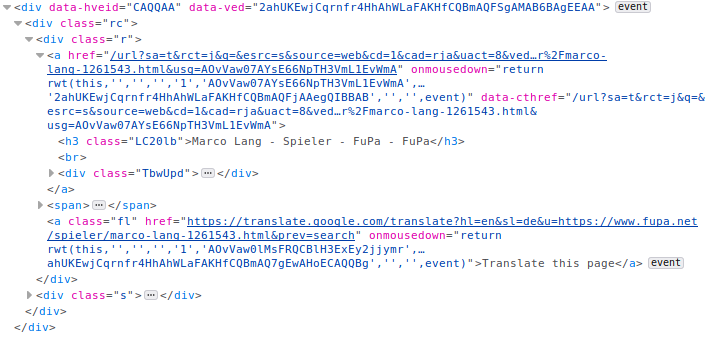
\includegraphics[ scale=0.7]{bilder/Google-Suchergebnis.png}
				\caption{Seitenquelltext von einem Google-Suchergebnis}
				\label{img:GoogleSeitenquelltext}
			\end{figure}
		
		Um zu erkennen, ob mehrere Seiten mit Suchergebnissen existieren, wird nach einer regular Expression in dem Link-Attribute  \textit{aria-label} gesucht. Die Regex suchen nach dem Wort \textit{Page}, welches von einer Nummer.

\section{Methoden zum Erkennen von wichtigen Informationen auf einer Webseite}
\label{subsec:ErkennenVonInformation}
Bei der Suche nach einer ausgewählten Person können verschiedenste Arten von Webseiten gefunden werden. Aus diesem Grund muss das Programm eine gewisse Intelligenz mit sich bringen um die wichtigsten Daten aus einer Seite herauszufiltern. Dabei ist es nicht möglich eine Hartkodierung zu verwenden, um festgelegte Bereiche einer Webseite auszulesen, da jede Webseite eine individuelle Struktur hat.\\
Die Grundidee zur Lösung diese Problems ist die Analyse des vorliegenden Webseiten-Textes. Eine Methode zur Textanalyse ist die automatisierte Schlüsselwort-Gewinnung. Hierbei wird die HTML-Seite zu einem verwendbaren Text formatiert, wobei die meisten Sonderzeichen herausgefiltert werden. Sonderzeichen wie "'."' und "'@"' werden dabei nicht herausgefiltert, da sie für die E-Mail-Erkennung wichtig sind. Anschließend werden Schlüsselwörter aus dem formatierten Webseitentext generiert. Möglichkeiten zur automatisierten Schlüsselwortgenerierung sind die Verfahren RAKE \ref{sec:RAKE} und die Automatic Keyword Extraction mit NLP \ref{sec:Automatic Keyword Extraction}, welche im Laufe dieser Arbeit detailliert beschrieben werden.\\
Nachdem die Schlüsselwörter generiert und in Listen gespeichert wurden, werden Wortsammlung erstellt. Diese Wortsammlungen sind Listen, welche aussagekräftige Schlüsselwörter enthalten und nach Themen kategorisiert werden. Beispiele für den Inhalt der Listen sind alle Hochschulen und Universitäten in Deutschland, Berufsbezeichnungen und Tätigkeiten, Studiengänge, Hobbybezeichnungen und alle Städte und Gemeinden in Deutschland.\\
Mit diesen Wortsammlungen kann nun die Liste mit den bereits generierten Schlüsselwörtern aus dem Webseitentext verglichen werden. Bei einer Übereinstimmung eines Schlüsselwortes wird das Wort mit der entsprechenden Kategorie vorgemerkt und später in die verwendete Speicherstruktur eingetragen. \\
Die Wortsammlungen werden mit Hilfe von bekannten Listen im Internet eigenständig befüllt. Als Informationsquelle dafür, dient jegliche Art von Webseite, die nützliche Information enthält.

	\subsection{RAKE}
	\label{sec:RAKE}
	RAKE steht für \textit{Rapid Automatic Keyword Extraction} und stellt eine sehr effiziente Methode zur Schlüsselwortgenerierung dar. Die Funktion von RAKE basiert darin, dass Schlüsselwörter mehrere Wörter mit inhaltlicher Relevanz enthalten, allerdings selten Stoppwörter und Sonderzeichen.\cite{rose2010automatic}\\
	Als Stoppwörter werden Wörter bezeichnet, die sehr oft auftreten und keinen großen Informationsgewinn mit sich bringen. Beispiele dafür sind \textit{und}, \textit{weil}, \textit{der} oder \textit{als}.\cite{Stopwords}\\
	
	\begin{figure}[h!]
		\fbox{\parbox{\linewidth}{In einer jungen Wissenschaft wie der Informatik mit ihrer Vielschichtigkeit und ihrer unüberschaubaren Anwendungsvielfalt ist man oftmals noch bestrebt, eine Charakterisierung des Wesens dieser Wissenschaft und Gemeinsamkeiten und Abgrenzungen zu anderen Wissenschaften zu finden. Etablierte Wissenschaften haben es da leichter, sei es, dass sie es aufgegeben haben, sich zu definieren, oder sei es, dass ihre Struktur und ihre Inhalte allgemein bekannt sind.}}
		\caption{Beispieltext}
		\label{fig:text}
	\end{figure}
	%TODO QUELLE für Beispieltext einfügen.
	
	Zu Beginn wird der zu analysierende Text, hier der Beispieltext in  Bild \ref{fig:text}, durch einen Worttrenner in ein Array, bestehen aus möglichen Schlüsselwörtern, aufgeteilt. Das erzeugte Array wird anschließend in Sequenzen von zusammenhängenden Wörtern unterteilt. Dabei erhalten die Wörter in einer Sequenz die gleiche Position und Reihenfolge wie im Ursprungstext und dienen gemeinsam als Kandidatenschlüsselwort.\cite{rose2010automatic}\\		
	Nachdem die möglichen Schlüsselwörter identifiziert sind, wird für jeden einzelnen Kandidaten ein Score ausgerechnet. Dieser besteht aus dem Quotient des Grades $deg(w)$ und der Häufigkeit des Vorkommens eines Wortes innerhalb der Kandidaten $freq(w)$. Daraus ergibt sich die Formel:
	\begin{center}
		$deg(w)/freq(w) $
	\end{center}	
	
	Dabei beschreibt der Grad eines Wortes, dass gemeinsame Auftreten mit sich selbst und anderen Schlüsselwörtern. In der Tabelle \ref{tab:Co-occurance} ist der Grad für jedes Wort ablesbar, indem die Einträge in der entsprechenden Reihe summiert werden. Beispielsweise Beträgt der Grad des Wortes \textit{"'Wissenschaft"'} den Wert \textit{3}. Dies ergibt sich aus der Rechnung:
	\begin{center}
		$2 + 1 = 3$
	\end{center}
	Das Wort \textit{"'Wissenschaft"'} kommt hier selbst zweimal in dem Kandidaten-Array vor und davon einmal in Verbindung mit dem Worten "'jungen"'.\\
	Die Häufigkeit des Vorkommens eines Wortes lässt sich ebenfalls in der Tabelle \ref{tab:Co-occurance} ablesen. Allerdings muss hier in der Reihe und Spalte des jeweiligen Wortes nachgeschaut werden. Für das Wort \textit{"'Wissenschaft"'} beträgt die Häufigkeit des Vorkommens den Wert \textit{3}.\\
	Zusammenfassend kann gesagt werden, dass \textit{deg(w)} die Kandidaten bevorzugt, welche oft und in langen Schlüsselwörtern, die mehrere Wörter enthalten, vorkommen. Dies bedeutet, dass beispielsweise \textit{deg(etabliert)} eine höhere Bewertung als \textit{deg(informatik)} bekommt, obwohl beide Wörter gleich oft im Text vorkommen. Dagegen wird bei \textit{freq(w)}, ausschließlich die Häufigkeit des Vorkommens bewertet. Bei der Formel \textit{deg(w)/freq(w)} werden die Wörter bevorzugt, welche überwiegend in langen Kandidatenwörtern vorkommen. Diese Formel bietet dadurch einen guten Mittelweg zur Schlüsselwortgewinnung. Ein Beispiel dafür sind die Wörter \textit{"'Wissenschaften} und \textit{"'allgemein"'}. Hier ist der Quotient von \textit{deg(allgemein)/freq(allgemein)} höher als von \textit{deg(Wissenschaften)/freq(Wissenschaften)}, obwohl die Häufigkeit des Wortes \textit{"'Wissenschaften"'} höher und der Grad gleich hoch ist. \cite{rose2010automatic}
	%TODO Möglicherweise kann Tabelle mit deg(w), freq(w) und deg(w)/feq(w)
	
	Durch das genannte Verfahren und der Formel \textit{deg(w)/freq(w)} für die Bewertung, ergeben sich die im Bild \ref{fig:SchlüsselwörterMitScore} befindenden Kandidaten mit den dazugehörigem Endbewertungen. \cite{rose2010automatic}
	
	\begin{center}
		\begin{table}[h!]
			\scriptsize
			\begin{tabular}{*{24}{l|}}				
				\rotatebox[origin=c]{90}{} 
				&\rotatebox[origin=c]{90}{wissenschaften} &\rotatebox[origin=c]{90}{wissenschaft} &\rotatebox[origin=c]{90}{sei} &\rotatebox[origin=c]{90}{etablierte} &\rotatebox[origin=c]{90}{informatik} &\rotatebox[origin=c]{90}{aufgegeben} &\rotatebox[origin=c]{90}{gemeinsamkeiten} &\rotatebox[origin=c]{90}{oftmals} &\rotatebox[origin=c]{90}{charakterisierung} &\rotatebox[origin=c]{90}{jungen} &\rotatebox[origin=c]{90}{inhalte} &\rotatebox[origin=c]{90}{allgemein} &\rotatebox[origin=c]{90}{bekannt} &\rotatebox[origin=c]{90}{struktur} &\rotatebox[origin=c]{90}{wesens} &\rotatebox[origin=c]{90}{bestrebt} &\rotatebox[origin=c]{90}{unüberschaubaren} &\rotatebox[origin=c]{90}{anwendungsvielfalt} &\rotatebox[origin=c]{90}{definieren} &\rotatebox[origin=c]{90}{abgrenzungen}
				&\rotatebox[origin=c]{90}{leichter}
				&\rotatebox[origin=c]{90}{finden}
				&\rotatebox[origin=c]{90}{vielschichtigkeit}\\
				\hline
				wissenschaften & 2 & & & 1 & & & & & & & & & & & & & & & & & & &\\
				\hline
				wissenschaft & & 2 & & & & & & & & 1 & & & & & & & & & & & & & \\
				\hline
				sei & & & 1 & & & & & & & & & & & & & & & & & & & &	\\
				\hline
				etablierte & 1 & & &1 & & & & & & & & & & & & & & & & & & &	\\
				\hline
				informatik & & & & &1 & & & & & & & & & & & & & & & & & & \\
				\hline
				aufgegeben & & & & & &1 & & & & & & & & & & & & & & & & &	\\
				\hline
				gemeinsamkeiten & & & & & & & 1& & & & & & & & & & & & & & & &	\\
				\hline
				oftmals & & & & & & & & 1& & & & & & & & & & & & & & &\\
				\hline
				charakterisierung & & & & & & & & & 1& & & & & & & & & & & & & & \\
				\hline
				jungen & & 1 & & & & & & & & 1 & & & & & & & & & & & & &	\\
				\hline
				inhalte & & & & & & & & & & & 1 & 1 & 1 & & & & & & & & & &	\\
				\hline
				allgemein & & & & & & & & & & & 1 & 1 & 1 & & & & & & & & & & \\
				\hline
				bekannt & & & & & & & & & & & 1 & 1 & 1 & & & & & & & & & &	\\
				\hline
				struktur & & & & & & & & & & & & & &1 & & & & & & & & &	\\
				\hline
				wesens & & & & & & & & & & & & & & &1 & & & & & & & &\\
				\hline
				bestrebt & & & & & & & & & & & & & & & & 1& & & & & & & \\
				\hline
				unüberschaubaren & & & & & & & & & & & & & & & & & 1 & 1 & & & & &	\\
				\hline
				anwendungsvielfalt & & & & & & & & & & & & & & & & & 1 & 1 & & & & &	\\
				\hline
				definieren & & & & & & & & & & & & & & & & & & & 1 & & & & \\
				\hline
				abgrenzungen & & & & & & & & & & & & & & & & & & & & 1 & & &	\\
				\hline
				leichter & & & & & & & & & & & & & & & & & & & & & 1 & &	\\
				\hline
				finden & & & & & & & & & & & & & & & & & & & & & & 1 & \\
				\hline
				vielschichtigkeit & & & & & & & & & & & & & & & & & & & & & & & 1	\\
				\hline
			\end{tabular}
			\label{tab:Co-occurance}
			\caption{Co-occurance}
		\end{table}
	\end{center}
	
	\begin{figure}[h!]
		\fbox{\parbox{\linewidth}{ inhalte allgemein bekannt (9.0), unüberschaubaren anwendungsvielfalt (4.0), jungen wissenschaft(3.5), etablierte wissenschaften (3.5), wissenschaften (1.5), wissenschaft (1.5), wesens (1.0), vielschichtigkeit (1.0), struktur (1.0), sei (1.0), oftmals (1.0), leichter (1.0), informatik (1.0), gemeinsamkeiten (1.0), finden (1.0), definieren (1.0), dass (1.0), charakterisierung (1.0), bestrebt (1.0), aufgegeben (1.0), abgrenzungen (1.0)}}
		\caption{Schlüsselwörter mit zugehörigem Score}
		\label{fig:SchlüsselwörterMitScore}
	\end{figure}
	\FloatBarrier

	\subsection{Automatic Keyword Extraction mit NLP}
	\label{sec:Automatic Keyword Extraction}
	Bei dieser Methode wird der vorliegende Text in die einzelnen Wörter unterteilt. Dabei wird eine Liste mit potentiellen Schlüsselwörtern erstellt, in der \textit{Stoppwörter} und Sonderzeichen herausgefiltert werden. Bei den Schlüsselwörtern handelt es sich nicht ausschließlich um ein Wort sondern auch um Wortsequenzen. Sogenannte N-Gramme bestehen aus einer festgelegten Anzahl von Wörtern. Dies hat den Vorteil, dass nicht nur Schlüsselwörter bestehend aus einem Wort erstellt werden können, sondern auch Schlüsselwörter mit Fragmenten eines Textes. Diese Art von Schlüsselwort wird benötigt um Informationen wie \textit{Hochschule Ravensburg-Weingarten} herauszulesen. Ein Beispiel-Trigramm, bei welchem ein Fragment drei Wörter beträgt, aus dem Beispieltext \ref{fig:text}  ist [\textit{'Wissenschaft und Gemeinsamkeiten'}].\\
	Erweiternd kann die Anzahl der Schlüsselwörter mit dem Verfahren von Stemming reduziert werden. Durch die Verwendung von ergänzende Regeln wie, eine Mindestanzahl von Buchstaben in einem Wort, können die Schlüsselwörter weiter begrenzen.

 

\section{Bewertung: Herausfiltern von wichtigen Informationen auf einer Webseite}
RAKE stellt eine fertige Methode dar, um Schlüsselwörter, die den Inhalt eines Textes in kurz wiedergeben, zu erstellen. Dabei hat ein Anwender kaum Möglichkeiten eigene Implementierungen vorzunehmen, da vieles vorgegeben ist. In der zu erstellenden Anwendung soll jedoch nicht der Inhalt eines Textes in Schlüsselwörter zusammengefasst werden, sondern es wird nach informationsreichen Wörtern gesucht. Aus diesem Grund ist jedes einzelne Wort aus dem Webseiten-Text von Bedeutung. Dies spricht gegen RAKE, da es nur die selbst errechnenden Favoriten-Schlüsselwörter zur Verfügung stellt. Dadurch werden viele Wörter nicht in Betracht gezogen oder für weiterführende Bearbeitungen bereitgestellt. Darüber hinaus ist die Berechnung eines Scores für diese Anwendung nicht notwendig.\\
Die Methode zur automatisierten Schlüsselwortgenerierung mit NLP bringt dagegen ein eigene Implementationsmöglichkeit mit sich. Das bedeutet, es kann selbst festgelegt werden, aus wie vielen Wörtern die Schlüsselwörter bestehen sollen. Des Weiteren wird jedes einzelne Wort in Betracht gezogen und verwendet. Die Suche nach einer E-Mail-Adresse im Text lässt sich allerdings bei beiden Methoden hinzufügen. Jedoch wird aus den eben genannten Vorteilen, die Information mit Hilfe der Methode zur automatisierten Schlüsselwortgewinnung mit NLP herausgefiltert.


\section{Umsetzung: Herausfiltern von wichtigen Informationen auf einer Webseite}
	\subsection{Text formatieren}
	Bevor die Schlüsselwörter generiert werden können, muss der Text in ein verwertbares Format umgewandelt werden. Aus diesem Grund wird der Seitenquelltext zuallererst mit Hilfe eines Python-Skripts namens html2text zu einem ASCII Plaintext umgewandelt.\cite{html2text} Anschließend werden Zeilenumbrüche und Sonderzeichen aus diesem Text herausgefiltert. Einzelne Wörter und Zahlen die weniger als 2 Zeichen haben, können ebenfalls aussortiert werden. Nachdem der Text in ein verwertbares Format umgewandelt wurde, kann mit der Umsetzung für die automatisierte Schlüsselwortgenerierung mit NLP begonnen werden.
	\subsection{Automatic Keyword Extraction}%TODO Muss noch festgelegt werden
	\subsubsection{Schlüsselwortgenerierung mit Python NTLK}
	Durch das \textit{Natural Language Toolkit} von Pyhton ist es möglich, den vorhandenen Webseitentext zu analysieren.\\
	Zu Beginn wird der vorhandene Text in einzelne Wörter zerlegt und in eine Liste gespeichert. Aus diesen Wörtern werden die "'stopwords"' der deutschen als auch der englischen Sprache herausgefiltert. Dadurch verringert sich die Anzahl der gesamten Wörter im Text um einen sehr großen Teil. \\
	Im nächsten Schritt werden die N-Gramme erstellt. Es werden nicht nur Bigramme sondern auch Trigramme, Tetragramme, Pentragramme und Hexagramme benötigt, damit vollständige Universitätsnamen und Firmennamen aus dem Text herausgelesen werden können. Alle erzeugten N-Gramme werden der eben erstellten Liste hinzugefügt. Diese Schlüsselwortliste wird später mit den Wortsammlungen verglichen.\\
	
	\subsection{Wortsammlungen erstellen}
	Es wäre denkbar, Datenbanken bzw. Wortsammlungen zu erstellen, welche die zu suchenden Schlüsselwörter beinhalten. Mit diesen Datenbanken kann nun die Liste mit den bereits verarbeiteten Wörter verglichen werden.
		\subsubsection{Wie werden Wortsammlungen befüllt?}
		 Die Datenbanken können mit Hilfe von bekannter Listen im Internet befüllt werden. Beispiele hierfür sind eine aktuelle Liste aller Hochschulen in Deutschland, Berufsbezeichnungen, Studiengänge, Hobbys, Städte und Gemeinden, etc..
		 Eingaben vom Anwender können ebenfalls eingefügt werden.
		\subsubsection{Wie werden sie am effektivsten verglichen?}

		
\section{Methoden zum Erkennen einer Person}
\label{sec:WannhandeltessichumdiegesuchtePerson}
Bei jeder einzelnen Suche, besteht die Herausforderung darin, zu erkennen, wann es sich um die gesuchte Person handelt. Durch die große Anzahl an verfügbaren Informationen im Internet, besteht eine hohe Wahrscheinlichkeit, dass Personen mit sehr ähnlichen Profilen gefunden werden.\\
Aus diesem Grund müssen Maßnahmen getroffen werden, damit die gesuchte Person erkannt wird. Dafür ist der erste Schritt die Anzahl der Suchergebnisse zu reduzieren. Dies ist durch den Ansatz der Personensuche im Kapitel \ref{sec:Suche nach Information} möglich. Dabei wird abhängig von der eingegebenen Information die Suche variiert. Des Weiteren kann durch eine Optimierung des Such-URLs \ref{subsubsec:URLOptimieren}, die Personensuche verfeinert und somit die Ergebnisse verbessert werden. Durch diese Maßnahmen steigt die Wahrscheinlichkeit, dass es sich um die richtige Person handelt.\\
Als zweites können die nachstehenden Methoden verwendet werden. Im Fall das auch mit diesen Methoden nicht die gesuchte Person identifiziert werden kann, können mehrere Personenprofile erstellt und angezeigt werde. Der Programm-Anwender kann anschließend aus den vorgeschlagenen Profilen eines auswählen.
	
	\subsection{Zeitraum beachten}
	Eine Methode für das Erkennen von Personen kann das Beachten von Zeiträumen sein. Dabei fließt das Alter der Zielperson mit in die Suche ein. Das bedeutet, dass nach dem Alter der Webseite gesucht wird, indem Jahreszahlen aus dem Webseitentext ausgelesen werden. Dadurch wird erkannt, ob der Zeitrahmen des Artikels oder das Erstellungsdatum einer Webseite mit dem Alter der Person grundsätzlich übereinstimmt.
%TODO Erklären wie man Zeitpunkt des Eintrages oder Alter der Webseite erkennen kann.

	\subsection{Kontakte der Suchperson werden in Betracht gezogen}	
	Hier kann die Suche erweitert werden, indem auf soziale und berufliche Verbindungen der Zielperson eingegangen wird. Das heißt, dass bekannte Kontakte der gesuchten Person ebenfalls durchsucht und ausgewertet werden. In diesem Fall könnten Facebook-Freunden, FuPa-Teammitglieder, Instagram-Follower oder LinkedIn/Xing-Kontakte als Kontaktquelle dienen.\\
	Durch dieses Verfahren können weitere Informationen gewonnen werden, die zur Unterscheidung von Profilen nützlich sein könnten.
	
	\subsection{Identifikationsschlüssel verwenden}
	Bekannte Information zur Person können als Identifikationsschlüssel verwendetet werden. Allerdings müssen dies einzigartige Daten sein. Als einzigartige Daten zählen beispielsweise die E-Mail-Adresse oder eine Verbindung von mehreren Daten. Der vollständige Name ist nicht einzigartig und dient deswegen nicht als Identifikationsschlüssel, da häufig verwendete Namen oft in Verbindung mit unterschiedlichen Personen im Internet vorkommen. Des Weiteren, kann eine Zielperson auf einer Webseite einen erfundenen Benutzernamen und auf der nächsten Seite den vollständigen Namen verwenden.\\
	

	
\section{Bewertung: Die gesuchten Person erkennen}
Grundsätzlich gilt, dass alle Methoden zur Erkennung einer Person eine Verbesserungen der Ergebnisse mit sich bringen. Allerdings gibt es Unterschiede in der Wirksamkeit und in der Laufzeit des Programms.
%TODO Bewertung schreiben
Die Erweiterung der Kriterien \ref{sec:ErweiterteKriteriern} bringt keine große Laufzeitänderung mit sich und stellt eine sehr gute Eigenschaft zur Optimierung der Informationsfindung dar, da die Zeit ebenfalls mit einbezogen wird.
\section{Umsetzung: Die gesuchte Person erkennen}
	\subsection{Zeitrahmen wird mit Beachtet}
		\subsubsection{Wie kann Alter der Webseite herausgefunden werden}
		Der Webseitentext kann nach Datums suchen und diese mit dem angegebenen Geburtsjahr verglichen werden. Dabei kann erkannt werden, ob das theoretische Alter des Artikels mit dem Alter der Person übereinstimmen kann. Möglicherweise können Metadaten von der Webseite ausgelesen werden.
	\subsection{Kontakte in Betracht ziehen}
		\subsubsection{Auf welcher Seite können mögliche Kontakte gefunden werden}
		Beinahe jede Social-Media-Seite bietet die Möglichkeit Kontakte der gesuchten Person anzusehen. Wenn nicht alle dann einen Teil
		\subsubsection{Wie werden Kontakte ausgelesen?}
		Möglicherweise hartkodiert.
	\subsubsection{Identifikationsschlüssel erstellen}
		\subsubsection{Was dient als Identifikationsschlüssel}
		E-Mail.

\section{Speicherung der gewonnenen Daten}
	Die gewonnenen Daten können in einem beliebig erweiterbaren Personen-Objekt gespeichert werden. Darüber hinaus lässt sich das Objekt mit bekannten Kontakten der zu suchenden Person erweitern.\\
	Eine andere Möglichkeit wäre die Daten in eine Datei auszulagern. Hierfür wäre eine Datei mit dem Format \textit{CSV} oder \textit{TXT} möglich.